
\documentclass[
   ngerman          % neue deutsche Rechtschreibung
  ,a4paper          % Papiergrösse
% ,twoside          % Zweiseitiger Druck (rechts/links)
% ,10pt             % Schriftgrösse
  ,11pt
% ,12pt
  ,pdftex
%  ,disable         % Todo-Markierungen auschalten
]{report}

\usepackage[utf8]{inputenc}        

\usepackage{dokumentation}

%% ACHTUNG, wenn man eine eigene Formatdatei (bericht.fmt) benutzt, werden Änderungen an bericht.sty
%% erst wirksam, wenn die Format-Datei neu erzeugt wurde!!!
%% Genauer alle Änderungen, die textuell vor der nächsten Zeile ".... endofdump...." stehen
%% werden erst wirksam, wenn die Formatdatei neu erzeugt wurde
\csname endofdump\endcsname

%%%%%%%%%%%%%%%%%%%%%%%%%%%%%%%%%%%%%%%%%%%%%%%%%%%%%%%%%%%%%%%%%%%%%%%%%%%%%%%
%% Angaben zur Arbeit
%%%%%%%%%%%%%%%%%%%%%%%%%%%%%%%%%%%%%%%%%%%%%%%%%%%%%%%%%%%%%%%%%%%%%%%%%%%%%%%

\newcommand{\Autor}{Toni Einecker}
\newcommand{\MatrikelNummer}{3523850}
\newcommand{\Kursbezeichnung}{Tinf18B3}
\newcommand{\FirmenName}{SICK AG}
\newcommand{\FirmenStadt}{Waldkirch}
\newcommand{\DhbwLogoDeckblatt}{
\includegraphics[width=4cm]{Bilder/dhbwLogo.PNG}}

%%%%%%%%%%%%%%%%%%%%%%%%%%%%%%%%%%%%%%%%%%%%%%%%%%%%%%%%%%%%%%%%%%%%%%%%%%%%%%

\newcommand{\Titel}{Dokumentation des Projekts}
\newcommand{\Was}{Wortfinder}
\newcommand{\AbgabeDatum}{17. Mai 2021}
\newcommand{\Abschluss}{Bachelor of Science}
\newcommand{\Studiengang}{Informatik / Informationstechnik}

\hypersetup{%%
  pdfauthor={\Autor},
  pdftitle={\Titel},
  pdfsubject={\Was}
}

%%%%%%%%%%%%%%%%%%%%%%%%%%%%%%%%%%%%%%%%%%%%%%%%%%%%%%%%%%%%%%%%%%%%%%%%%%%%%%%

\includeonly{
 kapitel1,
 kapitel2,
 kapitel3,
 kapitel4,
 kapitel5,
 anhang
}
%%%%%%%%%%%%%%%%%%%%%%%%%%%%%%%%%%%%%%%%%%%%%%%%%%%%%%%%%%%%%%%%%%%%%%%%%%%%%%%
%% Titelseite
%%%%%%%%%%%%%%%%%%%%%%%%%%%%%%%%%%%%%%%%%%%%%%%%%%%%%%%%%%%%%%%%%%%%%%%%%%%%%%%

\begin{document}
\begin{titlepage}
\begin{center}
\vspace*{-2cm}
%\FirmenLogoDeckblatt
\hfill\DhbwLogoDeckblatt\\[2cm]
{\Huge \Titel}\\[1cm]
{\Huge\scshape \Was}\\[1cm]
{\large für die Prüfung zum}\\[0.5cm]
{\Large \Abschluss}\\[0.5cm]
{\large des Studienganges \Studiengang}\\[0.5cm]
{\large an der}\\[0.5cm]
{\large Dualen Hochschule Baden-Württemberg Karlsruhe}\\[0.5cm]
{\large von}\\[0.5cm]
{\large\bfseries \Autor}\\[1cm]
{\large Abgabedatum \AbgabeDatum}
\vfill
\end{center}
\begin{tabular}{l@{\hspace{2cm}}l}
Matrikelnummer	                 & \MatrikelNummer		\\
Kurs			         & \Kursbezeichnung		\\
\end{tabular}
\end{titlepage}

%%%%%%%%%%%%%%%%%%%%%%%%%%%%%%%%%%%%%%%%%%%%%%%%%%%%%%%%%%%%%%%%%%%%%%%%%%%%%%%
%% Verzeichnisse
%%%%%%%%%%%%%%%%%%%%%%%%%%%%%%%%%%%%%%%%%%%%%%%%%%%%%%%%%%%%%%%%%%%%%%%%%%%%%%%

\pagenumbering{Roman}
\newpage
\tableofcontents

%%%%%%%%%%%%%%%%%%%%%%%%%%%%%%%%%%%%%%%%%%%%%%%%%%%%%%%%%%%%%%%%%%%%%%%%%%%%%%%
%% Inhalt
%%%%%%%%%%%%%%%%%%%%%%%%%%%%%%%%%%%%%%%%%%%%%%%%%%%%%%%%%%%%%%%%%%%%%%%%%%%%%%%
\cleardoublepage
\setcounter{savepage}{\arabic{page}}
\pagenumbering{arabic}
\chapter{Unit Tests}

Bei der Erstellung der Tests wurde auf die ATRIP-Regeln geachtet. Damit die Tests automatisch und wiederholbar sind, wurden sie mit xUnit erstellt und benötigen bei der Testausführung keinerlei Benutzerinteraktion. Dabei sind alle Tests unabhängig voneinander. Da sie gründlich erstellt wurden, existieren für die meisten Funktionen welche getestet werden mehrere Testfunktionen um möglichst alle Szenarien und auch Grenzfälle abzudecken. Außerdem wurde der Fokus auf Funktionen gelegt, welche für das Ausführen der Anwendung absolut notwendig sind. Dazu zählt hier vor allem das Generieren von Spielfeldern, das Auswählen von Wörtern und deren Überprüfung ob diese richtig sind.  


Die Tests wurden in der AAA-Normalform erstellt. Mock-Objekte wurden mit Moq erstellt. Ein Beispiel für die Normalform sowie die Verwendung von Mocks ist nachfolgend dargestellt. Dabei werden 5 Mocks erstellt, da diese im Konstruktor der Klasse benötigt werden und Anschließend eine Instanz der Klasse erzeugt. Danach wird die zu testende Funktion aufgerufen und anschließend überprüft ob das Ergebnis korrekt ist.

\begin{figure}[htb]
\centering
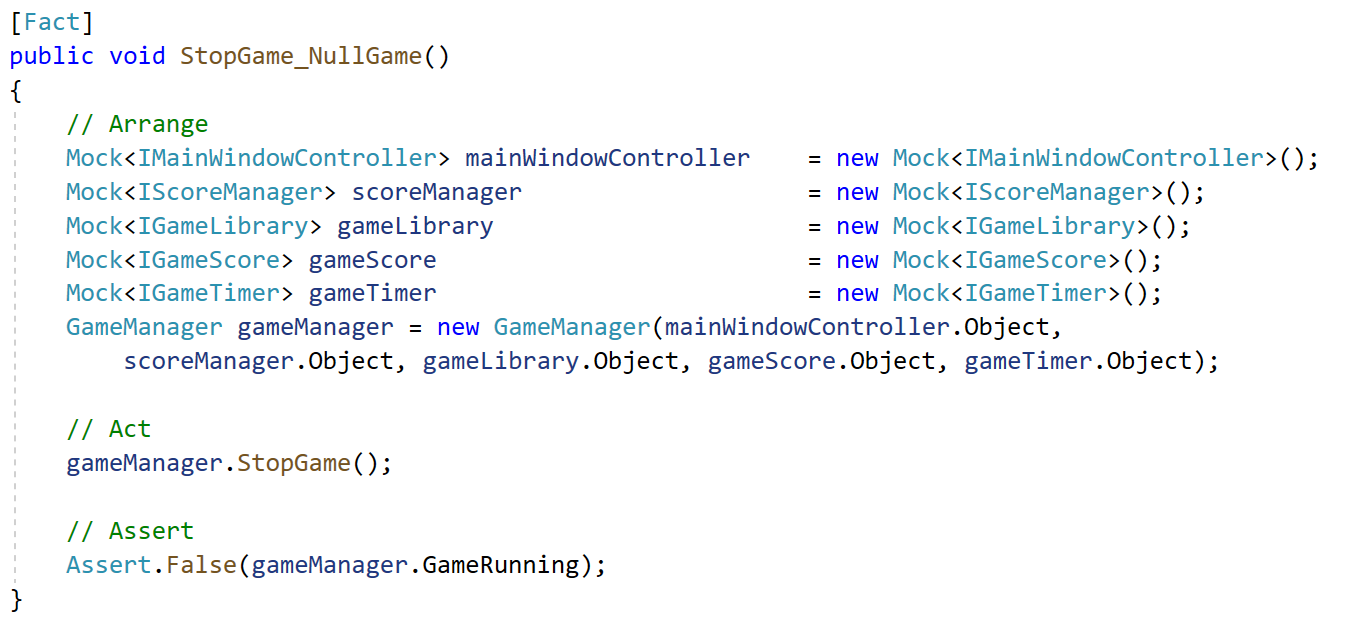
\includegraphics[width=0.7\textwidth]{Bilder/UnitTest.PNG}
\caption{\label{Abb:UnitTest}Beispiel Tests mit Mocks in AAA-Normalform}
\end{figure}



Die Testabdeckung beträgt 50\% Line Coverage.

\begin{figure}[htb]
\centering
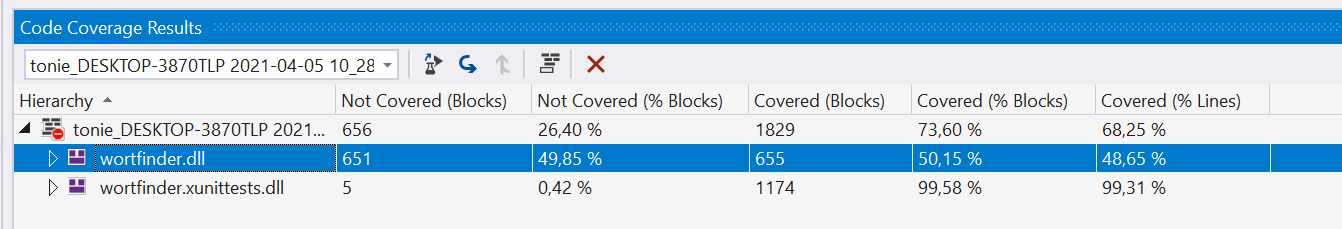
\includegraphics[width=1.0\textwidth]{Bilder/Testabdeckung.PNG}
\caption{\label{Abb:Testabdeckung}Die Ausgabe der Testabdeckung von Visual Studio}
\end{figure}

Die Abdeckung ist nicht höher, da ein Großteil der Codezeilen in den \textit{xaml} Dateien der GUI sind, welche nicht abgedeckt und nicht Unit Testbar sind. Außerdem sind primär die wichtigen Stellen im Quellcode mit Tests abgedeckt. Unwichtigere werden eher vernachlässigt.

\endinput
\chapter{Programming Principles}
\section{SOLID}
\paragraph{Single responsibility principle}
Die meisten Klassen in der Anwendung erfüllen das Prinzip. Eine Klasse welches es allerdings nicht erfüllt hat, ist der \textit{MainWindowController}. Dieser war zum einen der Adapter zwischen dem \textit{MainWindow} und dem \textit{GameManager} hat aber auch das verbinden von Buchstaben in der GUI kontrolliert. Die Funktionalitäten zum Verbinden von Buchstaben wurde daher in eine Neue Klasse \textit{WordBuilder} ausgelagert, Commit \href{https://github.com/EinToni/Wortfinder/commit/817e4b1b6be02defe58792a4afb709c7a147ced5}{817e4b1b6be02defe58792a4afb709c7a147ced5} und der darauf folgende. 


\paragraph{Open/Closed principle}
Eine auffällige Verbesserungsmöglichkeit wurde im \textit{GameScoreCalculator} gefunden, welcher immer wieder modifiziert wurde um die Punktzahl anders zu berechnen. Die Berechnung wurde nun Erweiterbar ausgelagert. Dafür wurde eine Liste im \textit{GameScoreCalculator} erstellt welche Klassen eines \textit{IPointFactor} Interfaces beinhaltet. Über diese wird beim Berechnen der Punkte Iteriert und jede Klasse berechnet dann einen Teilbetrag der Punktzahl, bezogen auf einen bestimmten Faktor. Siehe Commit \href{https://github.com/EinToni/Wortfinder/commit/6a4834cfc653a63ed3efc8745bccbe603250da74}{6a4834cfc653a63ed3efc8745bccbe603250da74}.


\paragraph{Liskov substitution principle}
Da keine Vererbung verwendet wird, ist das Liskov substitution principle erfüllt.

\paragraph{Dependency inversion principle}
Dependency inversion wurde im Rahmen der Implementierung der Clean Architecture an allen Grenzen der einzelnen Schichten angewendet.

\section{GRASP}
\paragraph{Grundkonzept} Der Code hat stellenweise eine recht hohe Kopplung, da oft Funktionen innerhalb der selben Klasse aufgerufen werden. Oftmals ist die Kopplung aber auch niedrig, weil für viele Klassen Interfaces verwendet und diese aufgerufen werden. Die Kohäsion ist vor allem im Domain und Application code recht hoch.


\paragraph{Code-Strukturierung}
Es wird viel Indirection verwendet. Ein gutes Beispiel dafür ist der \textit{GameManager}, welcher im Grunde alle aufrufe an verschiedene andere Klassen weiterleitet.


\paragraph{Architektur}
\glqq Pure fabrication\grqq{} findet sich in der \textit{EnDecoder} Klasse wieder. Diese ist unabhängig von jeglicher Anwendungslogik und ver- bzw. entschlüsselt einen beliebigen Stream mit einem beliebigen key in ein beliebiges Verzeichnis.


\paragraph{Entwurfsmuster}
Die GUI kommuniziert immer nur mit einen Controller. Ein Beispiel ist der \textit{MainWindowController}. Dieser Leitet die Aufrufe weiter und wandelt teilweise Datentypen um.


\section{DRY}
Das \glqq don't repeat yourself\grqq{} Prinzip wurde im Produktivcode meistens eingehalten, da die Informationen als Klassen Parameter gespeichert und wiederverwendet wurden. Somit ist die Information nur an einem Ort gespeichert. Innerhalb von Tests wurde das Prinzip allerdings häufig nicht eingehalten. Weil die Tests oft schnell geschrieben wurden, wurden meistens keine extra Variablen angelegt, sondern die Informationen mehrfach geschrieben. Die Anpassungen der Tests sind in Commit \href{https://github.com/EinToni/Wortfinder/commit/31e056a85512623173a8e4efa2faa828b2f66466}{31e056a85512623173a8e4efa2faa828b2f66466}.
\endinput
\chapter{Clean Architecture}

Zum implementieren der Clean Architecture wurde ein UML Diagramm erstellt (Abb.~\ref{Abb:CleanArchitectureBEFORE} im Anhang) um die aktuellen Abhängigkeiten zu sehen, dabei wurden ein paar Abhängigkeitspfeile weggelassen welche von weit außen nach innen gehen und die Lesbarkeit zu sehr verringern. 


Für die Struktur der Clean Architektur wurde sich auf 3 Schichten festgelegt, da die Funktionsweise des Programms recht simpel ist. Die innerste Schicht beinhaltet alle Entitäten welche zur strukturierten Datenspeicherung verwendet werden. Die mittlere Schicht umfasst die Anwendungslogik. Die äußere Schicht beinhaltet die Interaktion mit allem Außerhalb, d.h. die Controller zum lesen und schreiben der Daten auf der Festplatte sowie die GUI Elemente mit jeweiligen Controllern. 


\begin{figure}[!ht]
  \centering
  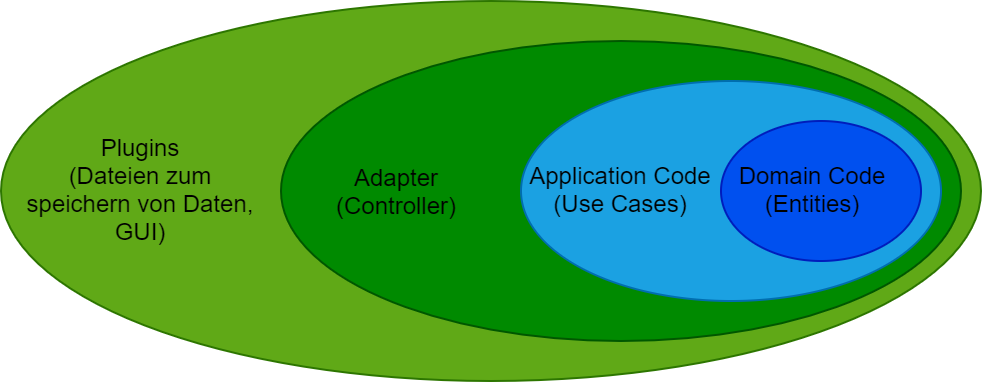
\includegraphics[width=0.6\textwidth]{Bilder/ArchitekturSchichten.PNG}
  \caption[Aufbau der Schichten der Clean Architecture]{Aufbau der Schichten der Clean Architecture \href{https://github.com/EinToni/WortfinderDoku/blob/main/Bilder/ArchitekturSchichten.png}{(link)}}
  \label{Abb:ArchitekturSchichten}
\end{figure}


Ein großes Problem sind hierbei Abhängigkeiten von Innen nach Außen, wie z.B. die \textit{WordFinder} Klasse (generiert alle möglichen Buchstabenkombinationen in einem Spielfeld), welche direkt auf den \textit{DataController} (nutzt die Wortliste auf der Festplatte) zu greift. Die Abhängigkeit wird durch Dependency Inversion, d.h. die Erstellung eines Interfaces welches die äußere Klasse implementiert und die innere nutzt, umgedreht \href{https://github.com/EinToni/Wortfinder/commit/586681478211a26abc661239ecc2c297ef77041e}{(link zum Commit)}:

\begin{figure}[!ht]
  \centering
  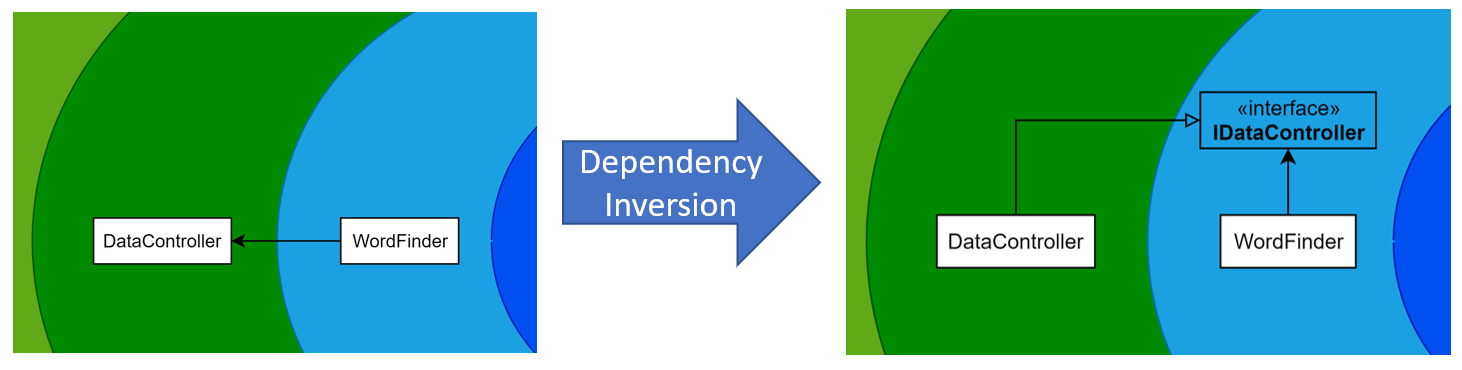
\includegraphics[width=0.8\textwidth]{Bilder/DependencyInversion.PNG}
  \caption[Beispiel der Dependency Inversion]{Beispiel der Dependency Inversion \href{https://github.com/EinToni/WortfinderDoku/blob/main/Bilder/DependencyInversion.png}{(link)}}
  \label{Abb:DependencyInversion}
\end{figure}

Wenn innere Klassen äußere erzeugen müssen, wie es beim \textit{WordFinder} der Fall ist, wird das Erzeugungsmuster der abstrakten Fabrik verwendet. Dem \textit{WordFinder} wird dann im Konstruktor eine Referenz auf die Fabrik gegeben. Über die Funktion "GetDataController()" gibt die Fabrik dann eine neue Instanz des \textit{DataController} zurück, wobei der Rückgabetyp im Interface der Fabrik als \textit{IDataController} Deklariert ist \href{https://github.com/EinToni/Wortfinder/commit/26148d6a7ae6784b935a260371672fe16f8bbfa0}{(link zum Commit)}:

\begin{figure}[!ht]
  \centering
  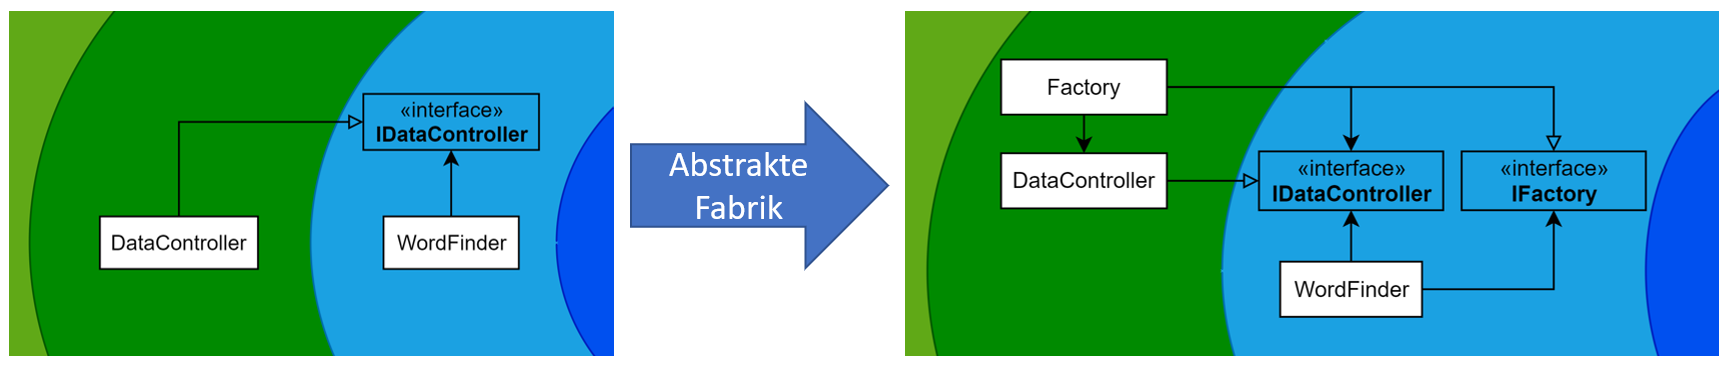
\includegraphics[width=0.8\textwidth]{Bilder/AbstrakteFabrik.PNG}
  \caption[Beispiel der Dependency Inversion]{Beispiel der Dependency Inversion \href{https://github.com/EinToni/WortfinderDoku/blob/main/Bilder/AbstrakteFabrik.png}{(link)}}
  \label{Abb:AbstrakteFabrik}
\end{figure}

Außerdem problematisch ist der grundsätzliche Aufbau der Programms sowie speziell der Aufbau des Hauptfensters. Dieses bestand aus einem Grid welches durch den \textit{FieldGenerator} mit Teilfenstern (\textit{LetterBox}, zeigen die Buchstaben an) gefüllt wurde. Jeder \textit{LetterBox} wurde die Instanz des \textit{WordBuilder} gegeben, welchen sie aufrufen wenn sie angeklickt werden.


Zur Verbesserung der Trennung zwischen dem Application Code und der GUI, wird das Grid direkt im Code Behind des \textit{MainWindow} durch kaskadieren von speziellen WPF  Elementen aufgebaut. Die Ansteuerung des \textit{MainWindow} erfolgt dann über einen neuen \textit{MainWindowController} dem im Aufruf nur die Größe des Spielfelds und die Buchstaben übergeben werden. Somit erfolgt die Erstellung der GUI separiert vom restlichen Anwendungscode.





Vor der Implementierung wurde zuerst das erstellte UML Diagramm abgeändert. Zuerst wurde dabei die Stuktur geändert, dann alle Abhängigkeitspfeile welche nach außen zeigen mittels Dependency Inversion umgedreht und als letztes an notwendigen Stellen eine Abstrakte Fabrik hinzugefügt. Das daraus entstandene Diagramm ist im Anhang als Abbildung~\ref{CleanArchitectureAFTER}.


Mit diesen Vorgaben wurde das Diagramm umstrukturiert, sodass alle Klassen an ihrem sinnvollsten Ort sind. Da das Programm vorher ständig mit Funktionen ergänzt wurde bei denen lediglich Wert auf Funktionalität gelegt wurde, sind im Nachhinein betrachtet unnötig komplizierte Strukturen entstanden. Diese werden daher bei der Umstrukturierung des Diagramms zur Clean Architecture auch gleich geändert. 
%% Beispiel für 
Ein Beispiel hierfür ist die \textit{FindableWords} Klasse, welche alle im aktuelle laufenden Spiel findbaren Wörter beinhaltet. Diese wurde erst später hinzugefügt, da davor direkt jedes Wort in einer Wortliste mit gültigen Wörtern überprüft wurde. Sowie die \textit{GameGrid} Klasse, welche (unter anderem) die Größe und Buchstaben des Spielfelds beinhaltet. Die findbaren Wörter sowie die Buchstaben im aktuellen Spiel wurden in eine neue Klasse \textit{Game} verschoben welche alle Daten über Spiel enthält. Somit können Spiele auch im Vorhinein generiert und dann geladen werden.

\endinput
\chapter{Code Smell Refactoring}

\subsection{Long Method}

Die Klasse \textit{WordGenerator} ist dafür zuständig alle möglichen Wörter in einem Raster von Buchstaben zu finden. Dafür hat sie zwei Funktionen welche jeweils ca. 50 Zeilen lang sind. Beide Funktionen sind durch viele Schleifen sehr unübersichtlich und fallen unter die Long Method Code Smells. Zum Refactoren des Code Smells wird die Funktion zuerst mittels Extract Method in kleinere Funktionen unterteilt. Dabei wurde direkt noch die If-Abfrage zur besseren Lesbarkeit umgedreht. Die extrahierten Methoden sind in Abb.\ref{Abb:ExtractMethod} in Grün und Orange markiert.\href{https://github.com/EinToni/Wortfinder/commit/b6e3b31e4ef7b597863bc2be073f9e136d4b9594}{(Link zum Commit)}

\begin{figure}[!ht]
  \centering
  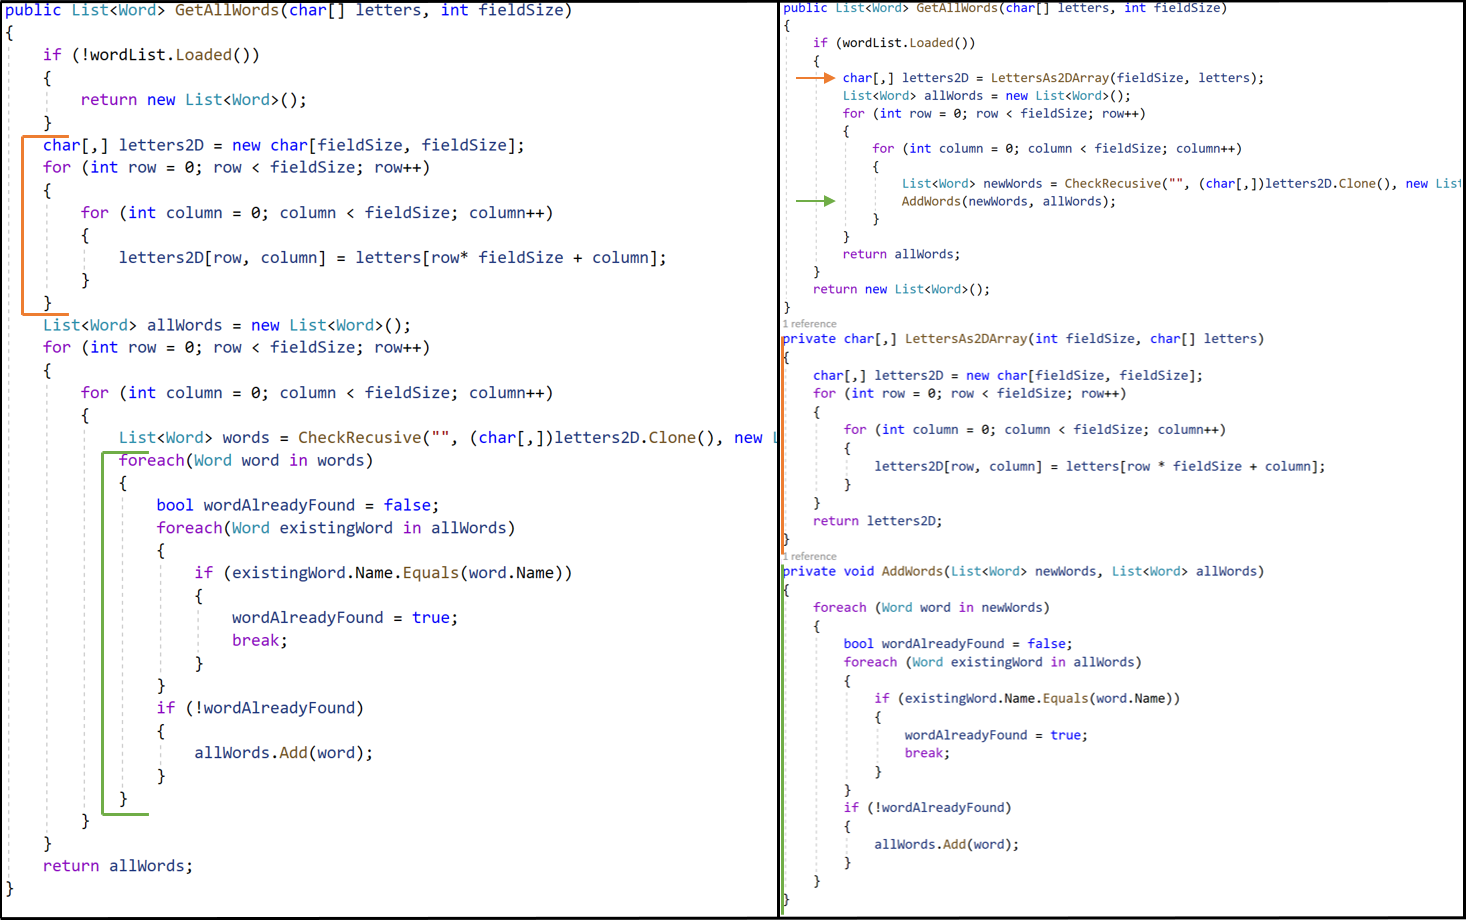
\includegraphics[width=\textwidth]{Bilder/ExtractMethod.PNG}
  \caption[Anwendung des Extract Method Refactoring]{Anwendung des Extract Method Refactoring \href{https://github.com/EinToni/WortfinderDoku/blob/main/Bilder/ExtractMethod.png}{(link)}}
  \label{Abb:ExtractMethod}
\end{figure}

Danach fallen die zwei gleichen Schachtelungen der for-Schleifen auf. Dabei wird in \textit{LettersAs2DArray} das Array zu einem 2D Array umstrukturiert, da die Buchstaben in einen Grid angeordnet sind ist so ein Iterieren und suchen von Nachbarn einfacher vorstellbar. Da zwischenzeitlich allerdings die \textit{Coordinate} Klasse eingefügt wurde, welche das Prüfen auf Nachbarschaft übernimmt, lässt sich dieser Code vereinfachen. Das durchlaufen des 2D Arrays (Abb.\ref{Abb:CodeVereinfachen} Orange markiert) wird somit durch ein einmaliges durchlaufen des Ursprünglichen Arrays ersetzt. Die \textit{LettersAs2DArray} Funktion wird hier nur noch für den Aufruf an die nächste Funktion benötigt und kann nach dessen Refactorings komplett entfernt werden. Außerdem kann die, in Grün markierte, Funktionalität welche überprüft ob ein Wort schon in der List ist ebenfalls durch Extract Method ausgelagert werden. Es ergibt sich somit folgender Code \href{https://github.com/EinToni/Wortfinder/commit/f733dabc6753529e597408cc8c76ea0a39a1ff8e}{(Link zum Commit)}:

\begin{figure}[!ht]
  \centering
  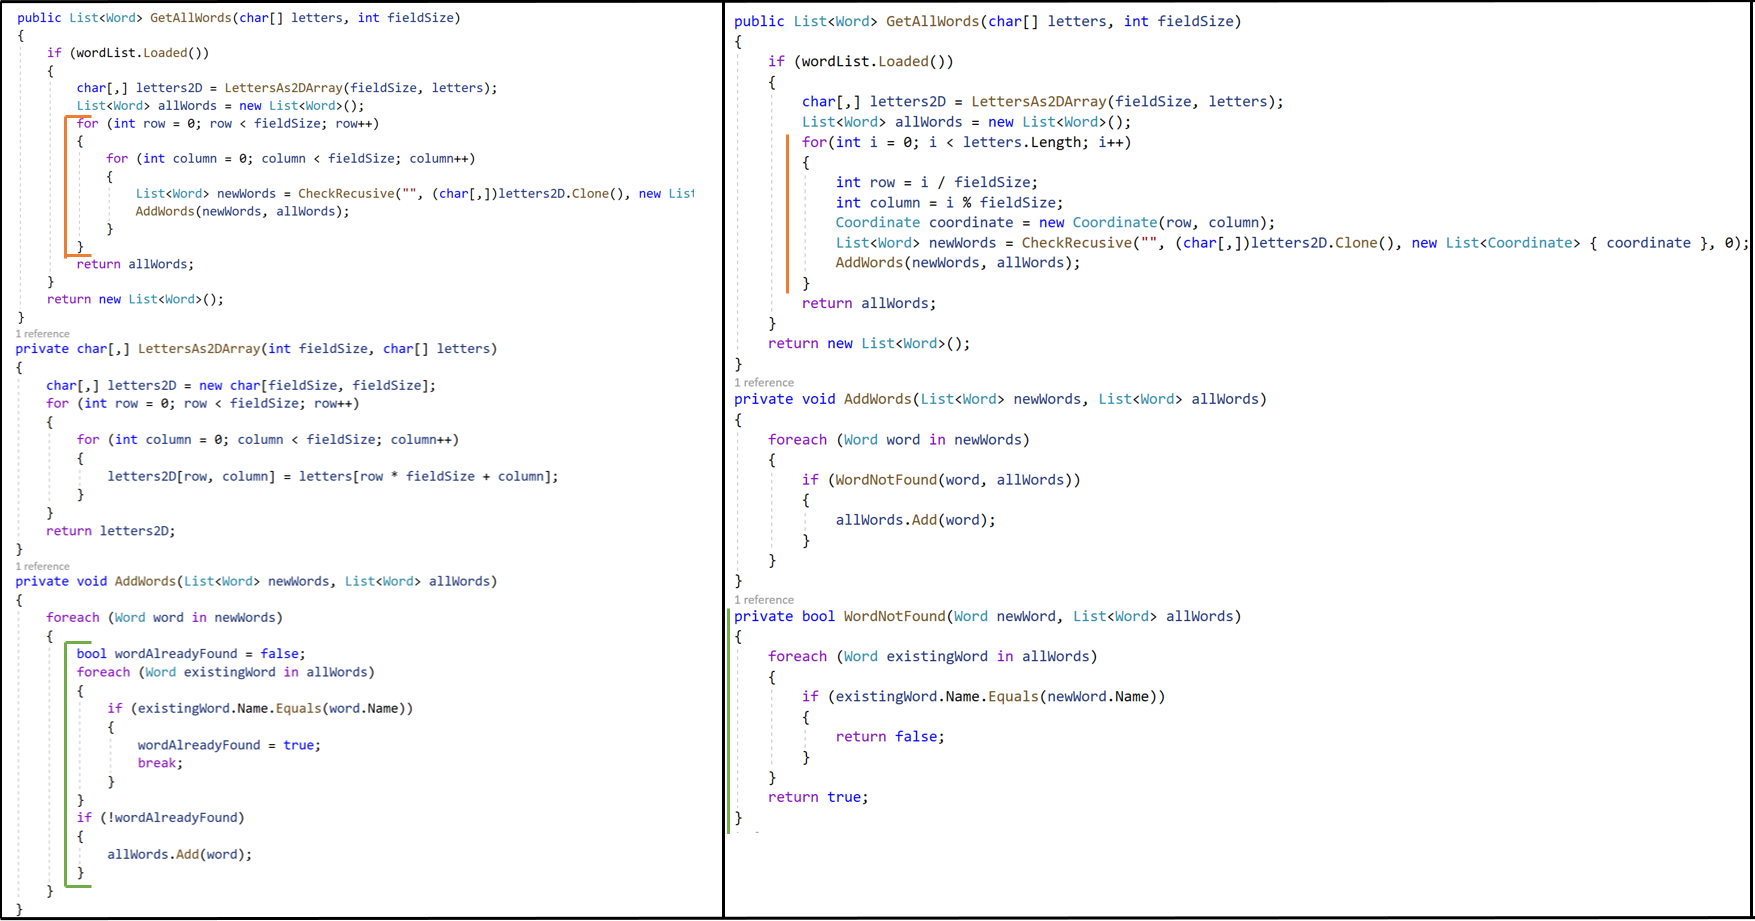
\includegraphics[width=\textwidth]{Bilder/CodeVereinfachen.PNG}
  \caption[Extract Method und Code Vereinfachung]{Extract Method und Code Vereinfachung \href{https://github.com/EinToni/WortfinderDoku/blob/main/Bilder/CodeVereinfachen.png}{(link)}}
  \label{Abb:CodeVereinfachen}
\end{figure}

In der zweiten Funktion wird ebenfalls mit Extract Method begonnen (Abb.\ref{Abb:ExtractMethod2}). Dabei werden zwei verschachtelte Schleifen ausgelagert, in welchen die betroffene Methode Rekursiv wieder aufgerufen wird. Da bei der Rekursion alle Parameter mitgegeben werden müssen ist ein komplettes auslagern unvorteilhaft, da in diese neue Methode dann ebenfalls alle Parameter weitergegeben werden müssten. Daher wird nur der Teil in eine neue Methode verschoben (Orange markiert), welcher alle benachbarten Positionen im Buchstabengitter findet \href{https://github.com/EinToni/Wortfinder/commit/23cf0b7d1165c1d17235d68f8fca35682ba233ad}{(Link zum Commit)}:

\begin{figure}[!ht]
  \centering
  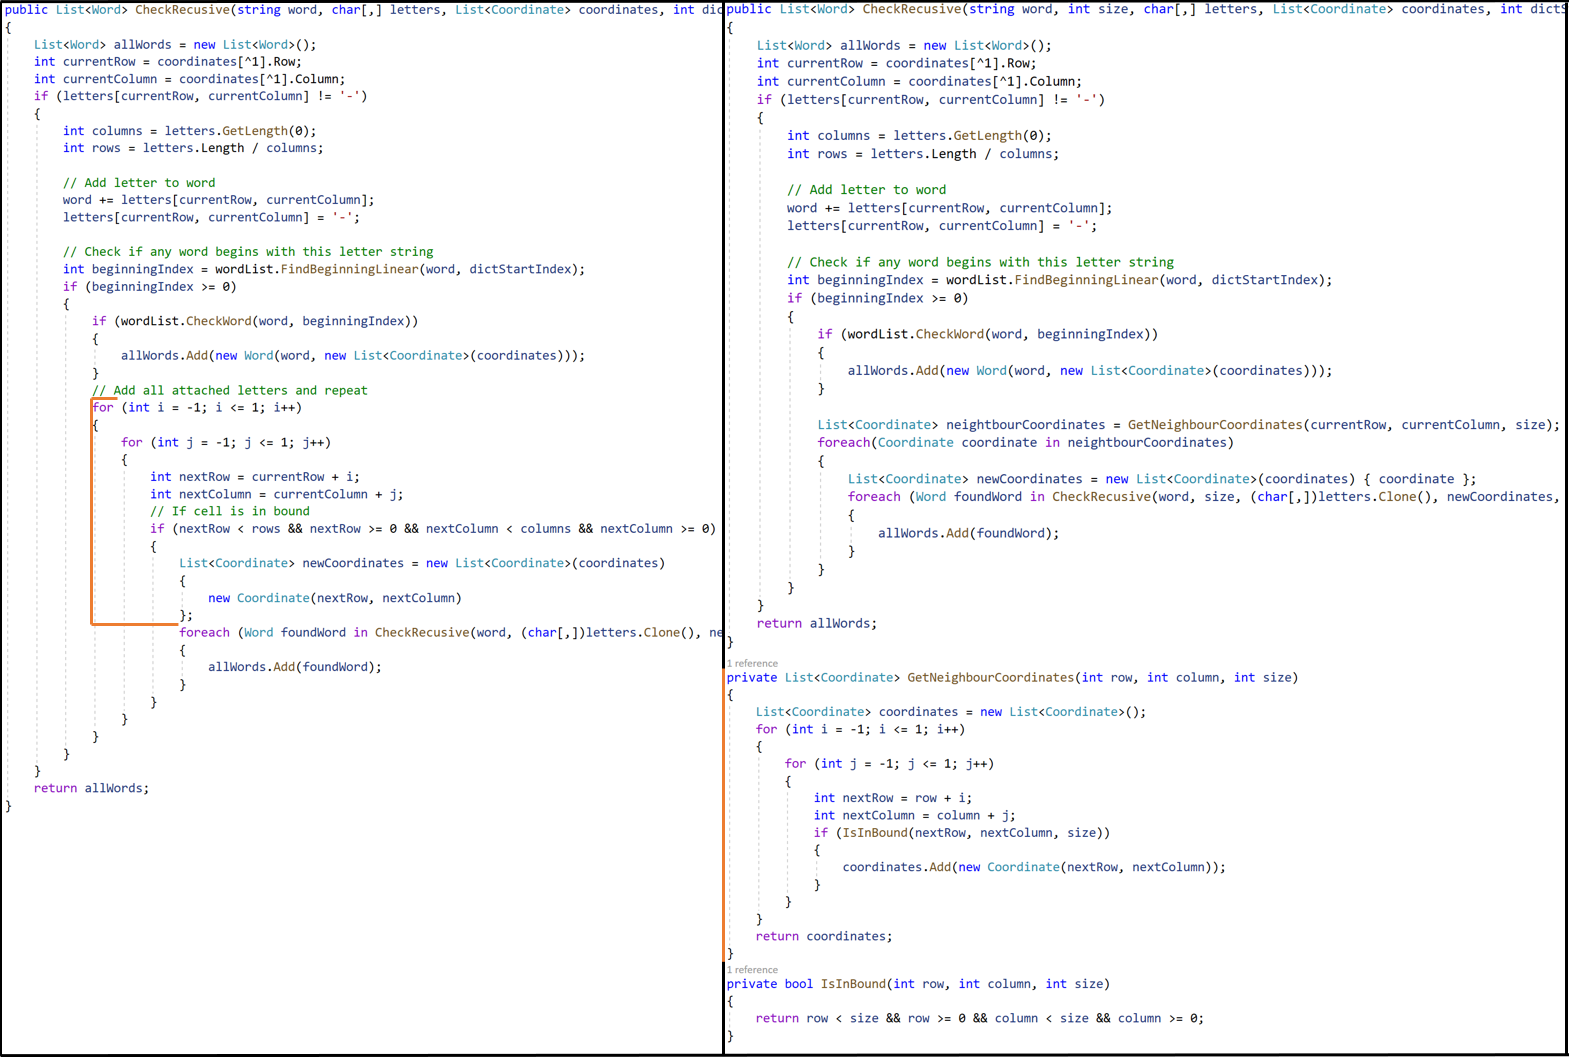
\includegraphics[width=\textwidth]{Bilder/ExtractMethod2.PNG}
  \caption[Extract Method]{Extract Method \href{https://github.com/EinToni/WortfinderDoku/blob/main/Bilder/ExtractMethod2.png}{(link)}}
  \label{Abb:ExtractMethod2}
\end{figure}

Danach wird auch hier das zweidimensionale Array durch ein eindimensionales ersetzt. Außerdem lässt sich das innerste foreach durch die Nutzung von der \textit{AddWords} Funktion ersetzen, welche durch Extract Method in der ersten Funktion entstand. 


Die Insgesamt Länge des Codes hat sich durch Anwenden der Refactorings nicht verkürzt. Dafür wurde die Lesbarkeit sowie die Wiederverwendbarkeit wesentlich gesteigert. Die fertigen Funktionen sind nachfolgenden Abgebildet \href{https://github.com/EinToni/Wortfinder/commit/e56ec221727039af2f0b6c06985f3b0edf8bdf3c}{(Link zum Commit)}:

\begin{figure}[!ht]
  \centering
  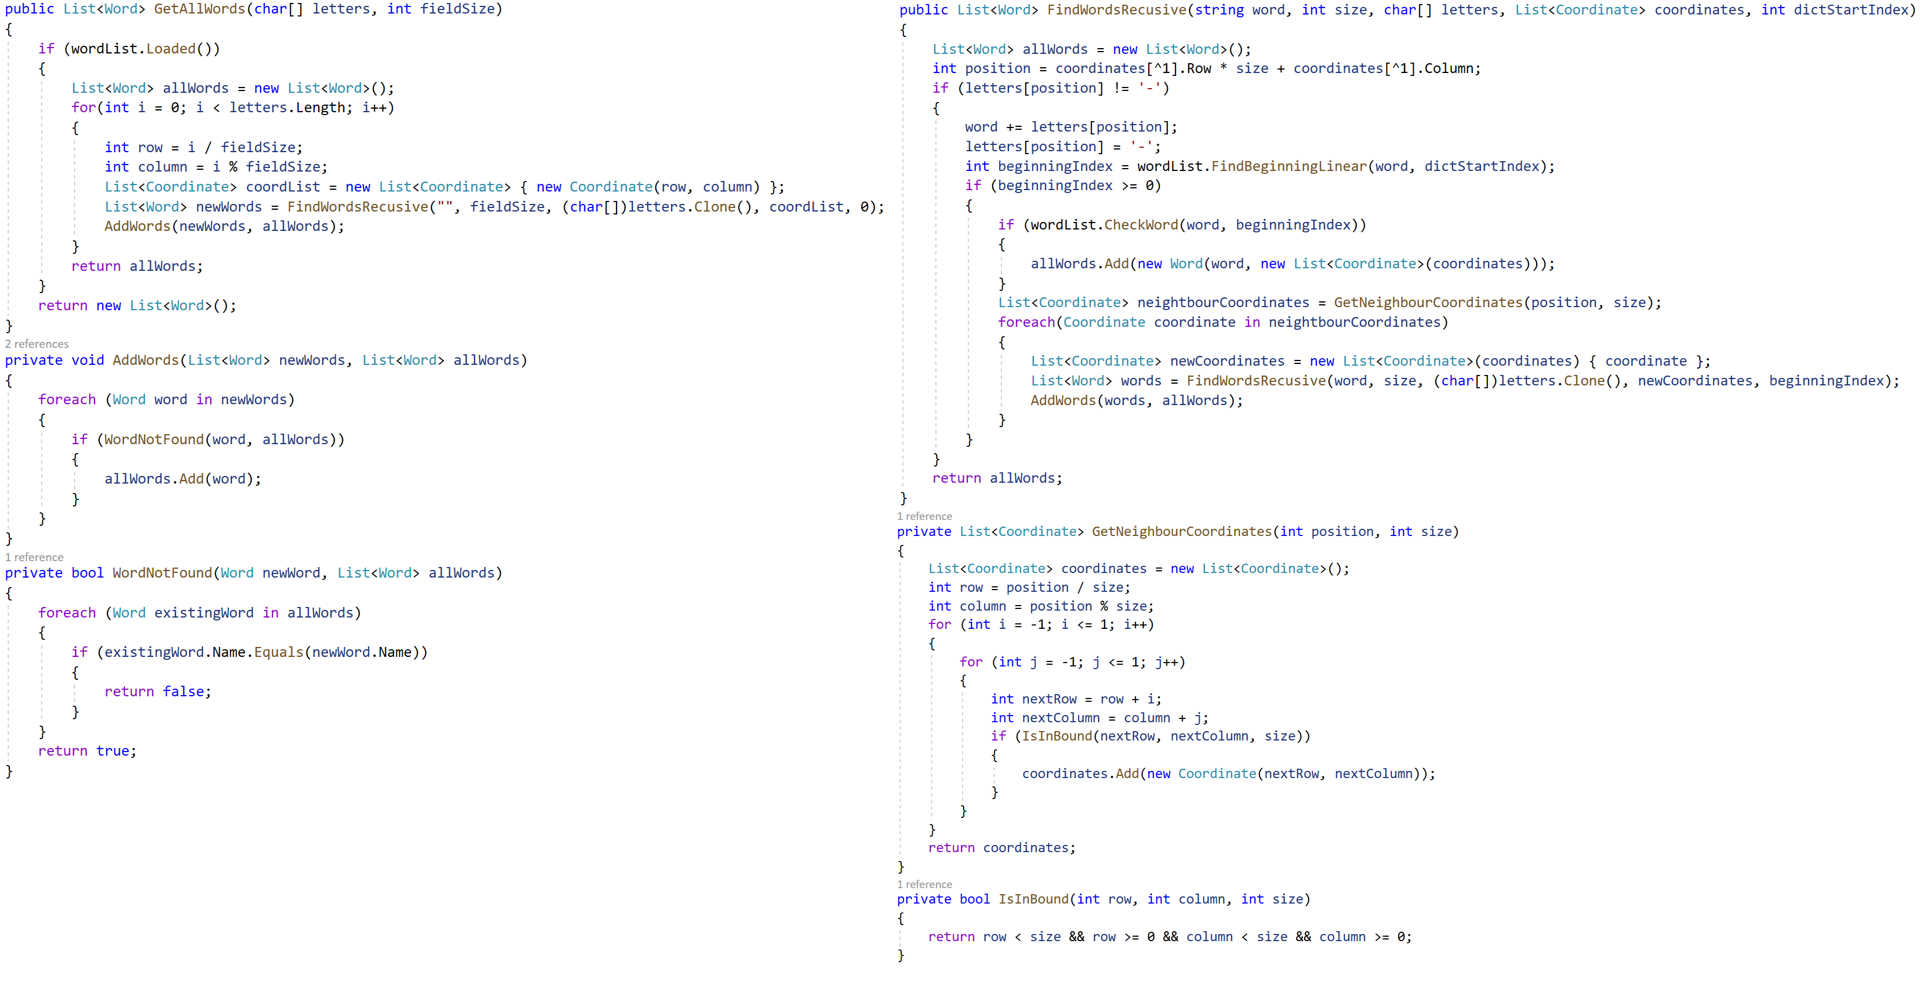
\includegraphics[width=\textwidth]{Bilder/endeRefactoring1.PNG}
  \caption[Long Method Code Smell nach dem Refactoring]{Long Method Code Smell nach dem Refactoring \href{https://github.com/EinToni/WortfinderDoku/blob/main/Bilder/endeRefactoring1.png}{(link)}}
  \label{Abb:endeRefactoring1}
\end{figure}

\subsection{Duplicated Code}

Es werden sowohl vorgeladenen Spiele, wie auch Highscores auf der Festplatte lokal gespeichert und beides soll nicht editierbar sein. Daher lädt und speichert die Klasse \textit{ScoreDataController} die Highscores sowie \textit{GameDataController} die vorbereiteten Spiele. Beide beinhalten dabei den gleichen Code für die Ent-/Verschlüsselung. Dieser Duplicated Code wird mittels Extract Method in eine neue Klasse ausgelagert welche die Ent- und Verschlüsselung übernimmt. \href{https://github.com/EinToni/Wortfinder/commit/86e635fc6ddbd436ca012c21e3a00b9246248855}{(Commit 86e635fc6ddbd436ca012c21e3a00b9246248855)}

\endinput
\chapter{Entwurfsmuster}

Ein im Quellcode des Programms identifiziertes Entwurfsmuster ist das des Beobachters. Dieses findet sich in der \textit{GameTimer} und \textit{GameManager} Klasse wieder. Der \textit{GameManager} registriert dabei zwei Callback-Funktionen beim \textit{GameTimer}. Nachdem der Timer gestartet wurde, wird die eine Funktion jede Sekunde, also jeden Tick des Timers, aufgerufen und die andere, sobald der Timer 0 erreicht. Der \textit{GameTimer} ist daher das Subjekt und der \textit{GameManager} der Beobachter.

Das UML Diagramm der beiden betroffenen Klassen ist nachfolgend abgebildet:

\begin{figure}[htb]
\centering
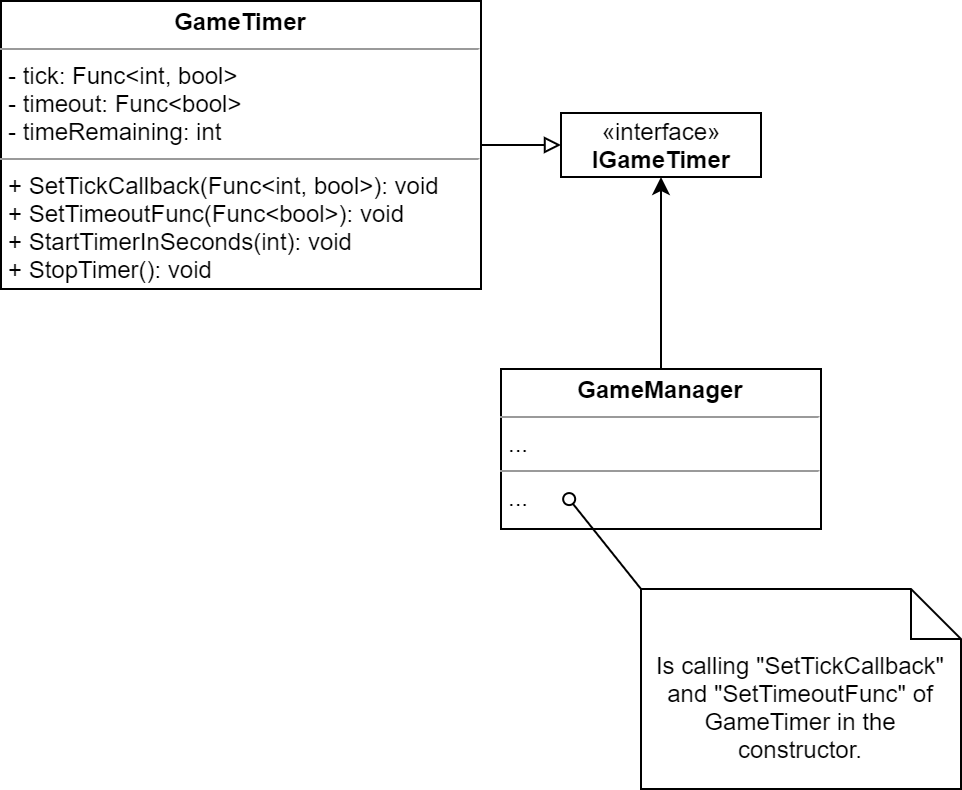
\includegraphics[width=0.7\textwidth]{Bilder/Entwurfsmuster.PNG}
\caption{\label{Abb:Entwurfsmuster}UML Diagramm des Beobachter Entwurfsmusters}
\end{figure}

\endinput

% Ab hier beginnt der Anhang
\appendix
\cleardoublepage
\pagenumbering{Roman}
\setcounter{page}{\thesavepage}
\addcontentsline{toc}{chapter}{Anhang}
\chapter{Abbildungen}

\begin{figure}[!ht]
  \centering
  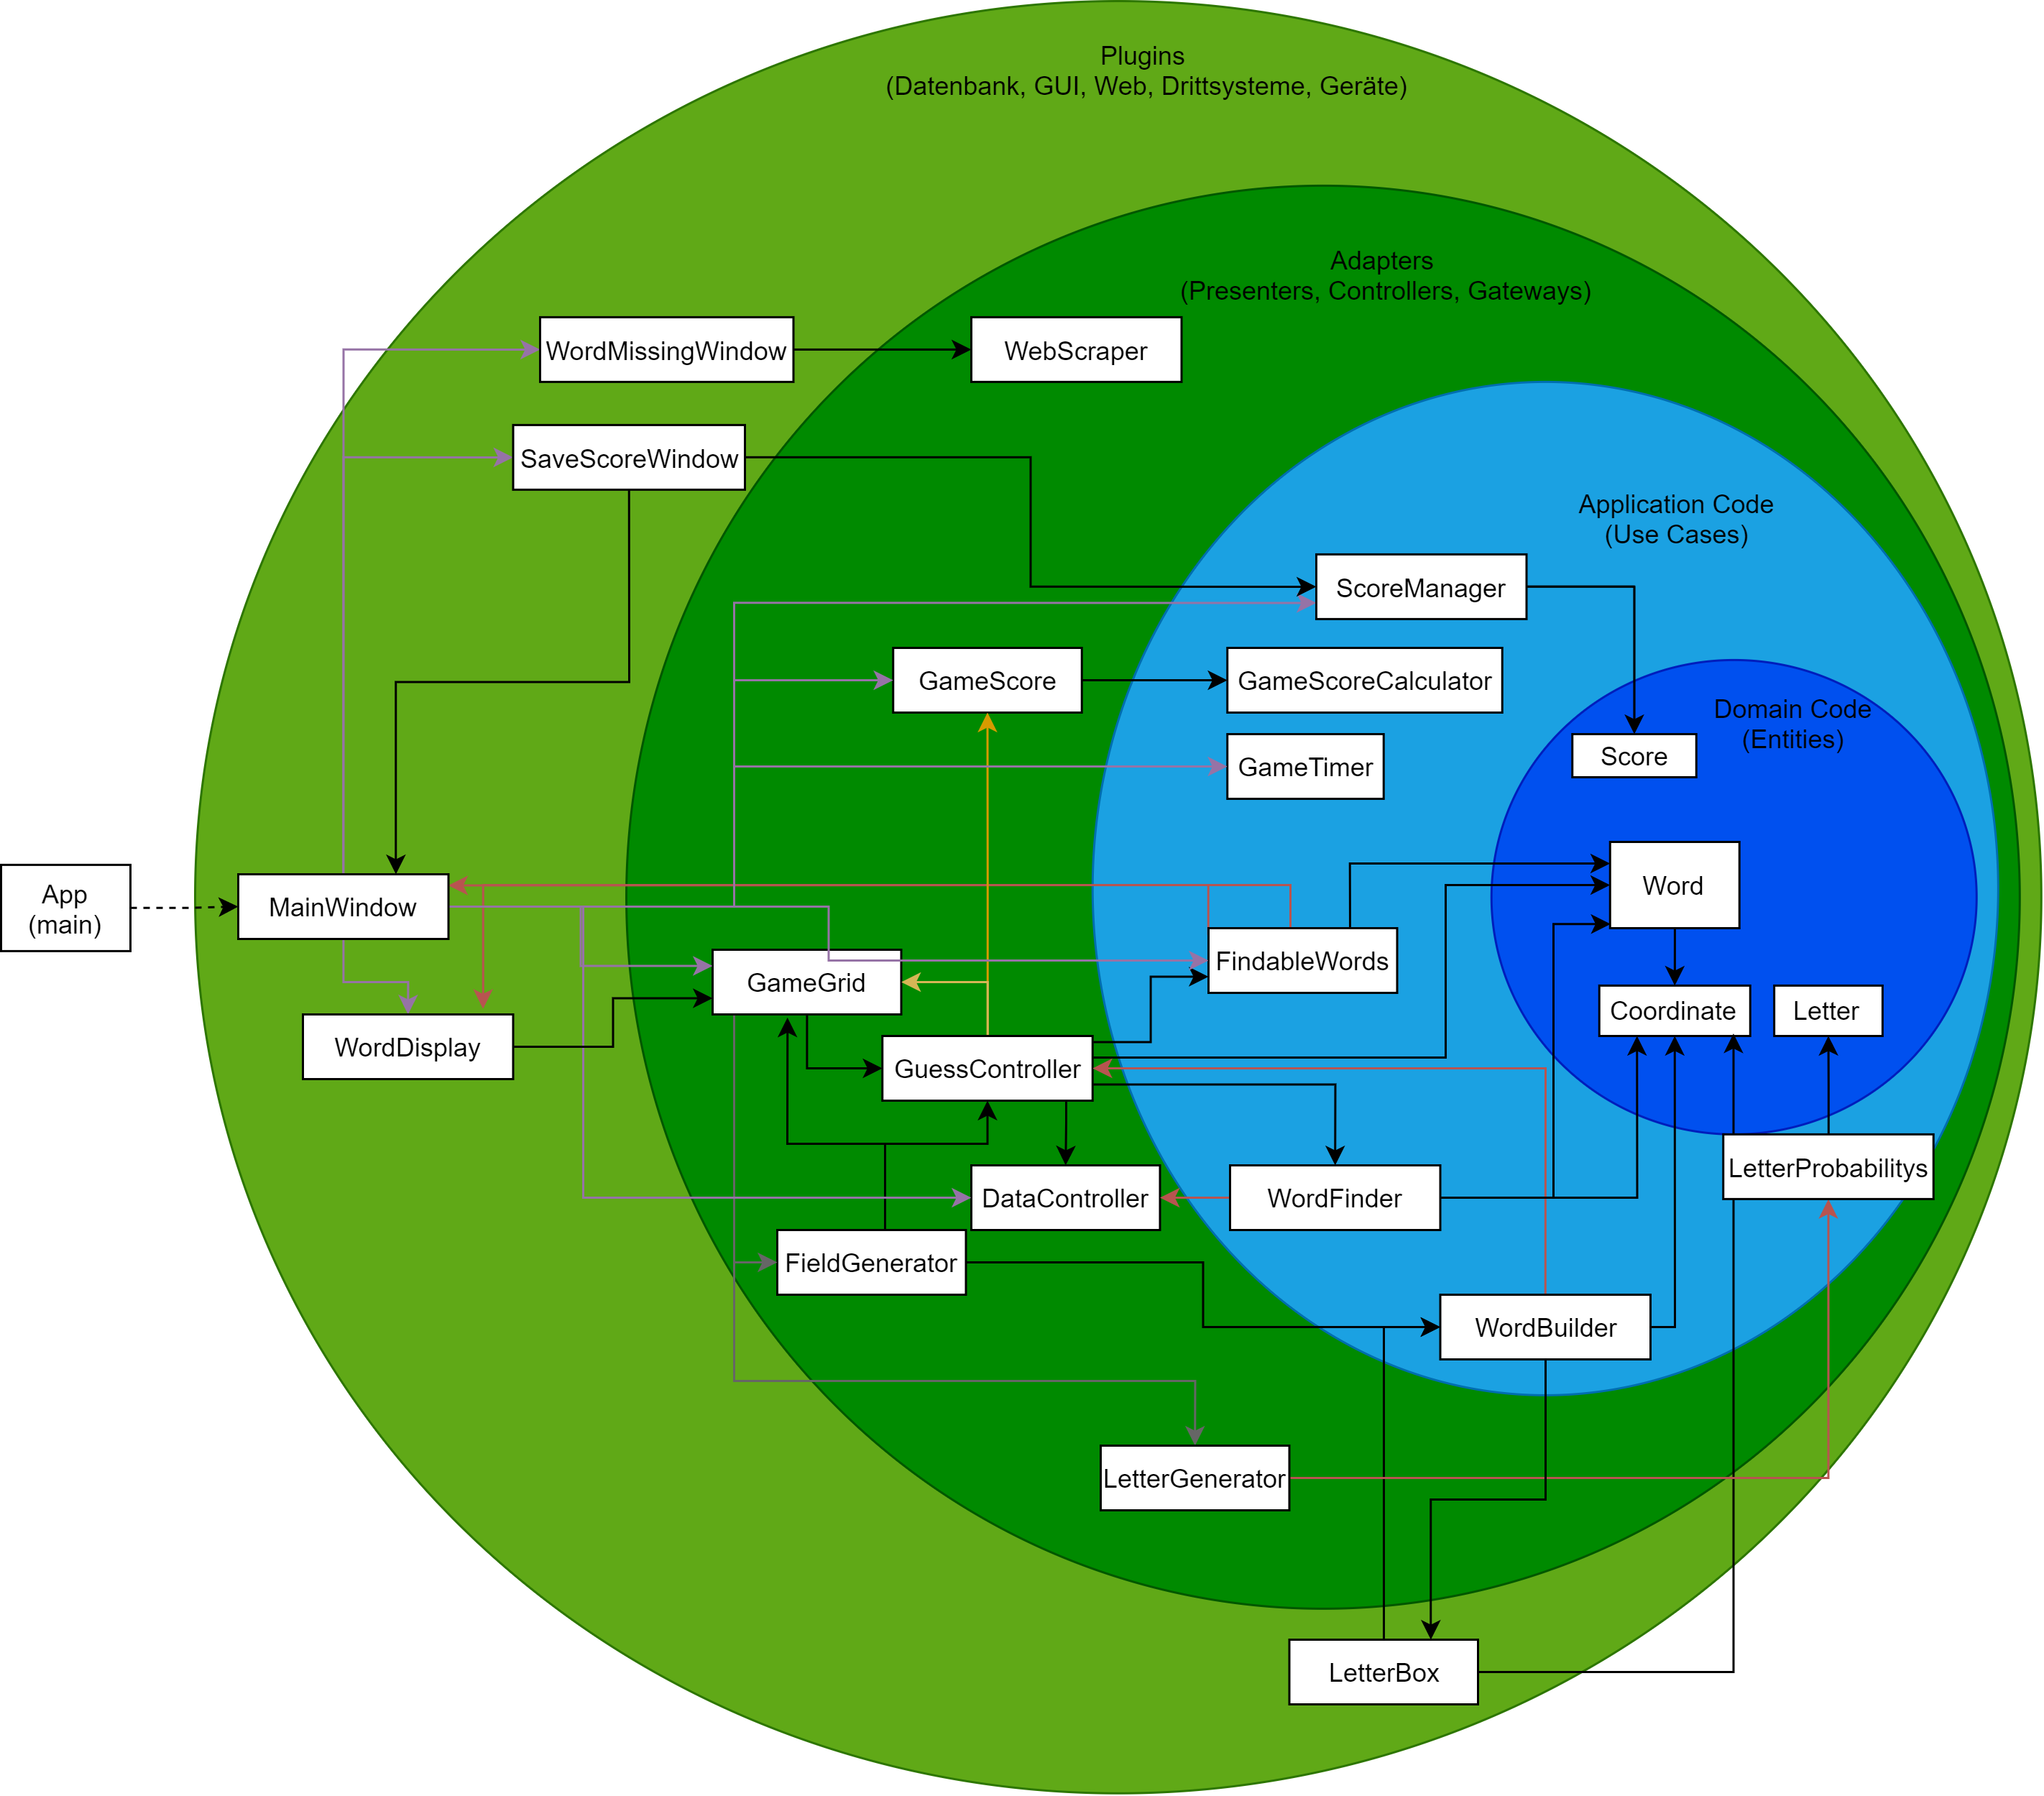
\includegraphics[width=0.9\textwidth]{Bilder/CleanArchitectureBEFORE.PNG}
  \caption[UML Klassendiagramm vor der Clean Architecture]{UML Klassendiagramm vor der Clean Architecture \href{https://github.com/EinToni/WortfinderDoku/blob/main/Bilder/CleanArchitectureBEFORE.png}{(link)}}
  \label{Abb:CleanArchitectureBEFORE}
\end{figure}

\begin{figure}[!ht]
  \centering
  \includegraphics[height=0.78\textheight, angle =90]{Bilder/CleanArchitectureAFTER.PNG}
  \caption[UML Diagramm nach der Clean Architecture]{UML Diagramm nach der Clean Architecture \href{https://github.com/EinToni/WortfinderDoku/blob/main/Bilder/CleanArchitectureAFTER.png}{(link)}}
  \label{Abb:CleanArchitectureAFTER}
\end{figure}

\begin{figure}[!ht]
  \centering
  \includegraphics[height=0.78\textheight, angle =90]{Bilder/CleanArchitectureAFTERinMain.PNG}
  \caption[UML Diagramm nach der Clean Architecture mit der Initialisierung in der Main]{UML Diagramm nach der Clean Architecture \href{https://github.com/EinToni/WortfinderDoku/blob/main/Bilder/CleanArchitectureAFTERinMain.png}{(link)}}
  \label{Abb:CleanArchitectureAFTERinMain}
\end{figure}

\endinput

\end{document}